\documentclass[a4paper,10pt]{book}

\usepackage[utf8]{inputenc}
\usepackage{amsmath}
\usepackage{amsfonts}
\usepackage{amssymb}
\usepackage{amsthm}
\usepackage[czech]{babel}
\usepackage{fontenc}
\usepackage{fancyhdr} %zahlavi a zapati
\usepackage{a4wide} % širší stránka
\usepackage{float} % obrázky na jedno místo
\usepackage{tikz}
\usepackage{listings}  % for source code (python\dots)
\usetikzlibrary {positioning}
\usepackage{tkz-euclide}
\usetkzobj{all}
\usetikzlibrary{calc,patterns}
\usetikzlibrary{intersections}
\usetikzlibrary{arrows,automata,shapes,quotes,decorations.markings}
\usepackage{tikz-3dplot}
\usepackage{newclude} % include bez clearpage
\usepackage{graphicx}
\usepackage{minted} % python code
\usepackage{multicol}
\usepackage{todonotes}
\usepackage{hyperref}
\usepackage[all]{hypcap}
\usepackage[parfill]{parskip}

% umožní vícestránkový align
\allowdisplaybreaks

% rejstřík
\usepackage{makeidx}
\makeindex

\title{Řešená cvičení z Matematické analýzy I}
\author{Jaroslav Hančl, Karel Král, Ondřej Pangrác a \url{https://kam.mff.cuni.cz/~sbirka/}}
\date{\today}

% theory macro
\newcommand{\theory}[1]{
	%\begin{center}
		%\line(1,0){250}
	%\end{center}
	%\newline % tady to dělá neplechu
	#1
}

\begin{document}
% Definitions
\newtheorem{theorem}{Věta}
\newtheorem{lemma}[theorem]{Lemma}
\newtheorem{conjecture}[theorem]{Domněnka}
\newtheorem{observation}[theorem]{Pozorování}
\newtheorem{corollary}[theorem]{Důsledek}
\newtheorem*{definition}{Definice}
%\theoremstyle{definition}\newtheorem*{define}{Definice}

 \maketitle

 \vskip 1cm

 Tento text není určen k šíření.
 Všechny chyby v tomto textu jsou samozřejmě záměrné. Reportujte je prosím na adresu
 {\tt kralka@iuuk.mff.cuni\ldots}.

 \vskip 2cm
 \tableofcontents

 \newcommand{\dx}{\ dx}
 \newcommand{\dt}{\ dt}
 \newcommand{\ds}{\ ds}
 \newcommand{\du}{\ du}
 \newcommand{\dv}{\ dv}

 \newcommand{\dif}{\, \mathrm{d}} % put at the beginning of document
 \newcommand{\id}{\, \mathrm{id}} % put at the beginning of document
 \newcommand{\sgn}{\, \mathrm{sgn}} % put at the beginning of document
 \newcommand{\med}{\, \mathrm{med}} % put at the beginning of document
 \newcommand{\conv}{\, \mathrm{conv}} % put at the beginning of document
 \newcommand{\supp}{\, \mathrm{Supp}} % put at the beginning of document
 \newcommand{\Ker}{\, \mathrm{Ker}} % put at the beginning of document
 \renewcommand{\Im}{\, \mathrm{Im}} % put at the beginning of document
 \newcommand{\R}{\, \mathcal{R}} % put at the beginning of document
 % nastavíme použití toho stylu
  %\pagestyle{fancy}
 % fakt hloupý nápad, když chci rejstřík
 %\pagenumbering{gobble} % bez čísel stránek

	\eject

\chapter{Zadání}
	% solution macro, this does NOT prints the solution
	\newcommand{\solution}[1]{}
	\newcommand{\exercise}[2]{ % file, label
		\input{#1}

		Řešení: \ref{sol:#2}
	}
	\section[1. Cvičení]{Cvičení}
 \include*{s1}
	\section[2. Cvičení]{Cvičení}
 \include*{s2}
	\section[3. Cvičení]{Cvičení}
 \include*{s3}
	\section[4. Cvičení]{Cvičení}
 \include*{s4}
	\section[5. Cvičení]{Cvičení}
 \include*{s5}
	\section[6. Cvičení]{Cvičení}
 \include*{s6}
	\section[7. Cvičení]{Cvičení}
 \include*{s7}
	\section[8. Cvičení]{Cvičení}
 \include*{s8}
	\section[9. Cvičení]{Cvičení}
 \include*{s9}
	\section[10. cvičení]{cvičení}
 \include*{s10}
	\section[11. cvičení]{cvičení}
 \include*{s11}
	\section[12. cvičení]{cvičení}
 \include*{s12}
	\section[13. cvičení]{cvičení}
 \include*{s13}
	\section[14. cvičení]{cvičení}
 \include*{s14}

\chapter{Tahák}
	\section{Základní vlastnosti funkcí}
	\section{Logika}
		Negace výroků:
\begin{multicols}{2}
\begin{enumerate}
	\item  $\neg (\neg A) \equiv A$
	\item  $\neg (A \wedge B) \equiv (\neg A) \vee (\neg B)$
	\item  $\neg (A \vee B) \equiv (\neg A) \wedge (\neg B)$
	\item  $\neg (A \Rightarrow B) \equiv A \wedge (\neg B)$
	\item  $\neg (A \Leftrightarrow B) \equiv A \Leftrightarrow (\neg B)$
	\item  $\neg \left( \forall x \colon \varphi(x) \right) \equiv \exists x \colon \neg \varphi(x)$
	\item  $\neg \left( \exists x \colon \varphi(x) \right) \equiv \forall x \colon \neg \varphi(x)$
\end{enumerate}
\end{multicols}
Pozor na ``existuje právě jedno'': $\neg \left( \exists! x \colon \varphi(x) \right) \equiv \left( \forall x \colon \neg \varphi(x) \right) \vee \left( \exists x \exists y \colon x \neq y \wedge \varphi(x) \wedge \varphi(y) \right)$


	\section{Limity}
		\begin{definition}
	Nechť $(a_a) \subset \mathbb{R}, a \in \mathbb{R}$.
	Číslo $a$ je limitou posloupnosti $(a_n)$, psáno $\lim a_n = \lim_{n \rightarrow \infty} a_n = a$, když
	$$\forall \varepsilon > 0 \  \exists n_0 \in \mathbb{N} \  \forall n > n_0 \colon |a_n - a| < \varepsilon.$$
	\label{def:limita_vlastni}
\end{definition}


		\begin{theorem}[Bolzano-Weierstrass (BW)]
	Každá posloupnost $(a_n)_{n=1}^{\infty}$ má podposloupnost $(b_n)_{n=1}^{\infty}$, která je monotónní.
	\label{thm:bolzano_weierstrass}
\end{theorem}

\begin{theorem}[(EDL)]
	$\lim_{n \rightarrow \infty} a_n = a \Leftrightarrow \lim_{n \rightarrow \infty}(a_n - a) = 0 \Leftrightarrow \lim_{n \rightarrow \infty}|a_n - a| = 0$
	speciálně $\lim_{n \rightarrow \infty} a_n = 0 \Leftrightarrow \lim_{n \rightarrow \infty} |a_n| = 0$.
	\label{thm:edl}
\end{theorem}

\begin{theorem}[Věta o limitě podposloupnosti (VOVP)]
	Nechť $\lim_{n \rightarrow \infty} a_n = a \in \mathbb{R} \cup \left\{ -\infty, +\infty \right\}$ a $(b_n)$ je posloupnost vybraná z $(a_n)$.
	Pak $\lim_{n \rightarrow \infty} a_n = \lim_{n \rightarrow \infty} b_n$.
	\label{thm:veta_o_vybrane_posloupnosti}
\end{theorem}

\begin{theorem}[Věta o aritmetice limit (VOAL)]
	Nechť $a, b \in \mathbb{R} \cup \{\pm \infty \}$ a posloupnosti $(a_n), (b_n)$ splňují $\lim a_n = a$ a $\lim b_n = b$.
	Potom
	\begin{align*}
			\lim_{n \rightarrow \infty}(a_n \pm b_n) &= \lim_{n \rightarrow \infty} a_n \pm \lim_{n \rightarrow \infty} b_n = a \pm b \\
			\lim_{n \rightarrow \infty}a_nb_n &= \lim_{n \rightarrow \infty} a_n \cdot \lim_{n \rightarrow \infty} b_n = ab \\
			\lim_{n \rightarrow \infty}\frac{a_n}{b_n} &= \frac{\lim_{n \rightarrow \infty} a_n}{\lim_{n \rightarrow \infty} b_n} = \frac{a}{b} \mbox{ pro } b \not= 0
	\end{align*}
	pokud má pravá strana těchto rovností smysl.
	\begin{itemize}

			\item Smysl dává:
				$$t + \infty = \infty + t = \infty$$
				$$t - \infty = -\infty + t = -\infty$$
				$$t / \pm \infty = 0$$
				$$\infty + \infty = \infty \cdot \infty = \infty$$
				$$-\infty - \infty = -\infty$$
				$$(-\infty) \cdot (- \infty) = \infty$$
				kde $t \in \mathbb{R}$.

				Pro $t \in (0, \infty]$ máme
				$$t \cdot \infty = \infty \cdot t = \infty$$
				$$t \cdot (-\infty) = (-\infty) \cdot t = -\infty$$
				
				Pro $t \in [-\infty, 0)$ máme
				$$t \cdot \infty = \infty \cdot t = -\infty$$
				$$t \cdot (-\infty) = (-\infty) \cdot t = \infty$$

			\item Smysl nedává (a tedy nemůžeme použít tuto větu přímo, ale musíme dál přemýšlet -- laicky řečeno tady záleží jak jsou ta nekonečna velká, případně jak malé jsou ty nuly):
				$$\pm \infty / \pm \infty$$
				$$\mbox{cokoliv}/0$$
				$$\infty - \infty$$
				$$-\infty - (-\infty)$$
				$$0 \cdot (\pm \infty)$$

	\end{itemize}
	\label{thm:veta_o_aritmetice_limit}
\end{theorem}

\begin{theorem}[Věta o dvou policajtech]
	Nechť posloupnosti $(a_n), (b_n), (c_n) \subset \mathbb{R}$ splňují, že
	$$\underset{n \rightarrow \infty}{\lim} a_n = \underset{n \rightarrow \infty}{\lim} b_n = a \in \mathbb{R}$$
	a nechť existuje $n_0 \in \mathbb{N}$ takové, že pro každé $n > n_0$ platí $a_n \leq c_n \leq b_n$.
	Pak $(c_n)$ konverguje a navíc $\underset{n \rightarrow \infty}{\lim} c_n = a$.
	\label{thm:dva_policajti}
\end{theorem}

\begin{theorem}[Násobení limitní nulou (VOSON)]
	Nechť posloupnost $(a_n)$ je omezená a posloupnost $(b_n)$ konverguje k nule, pak $\lim_{n \rightarrow \infty} a_n \cdot b_n = 0$.
	\label{thm:nasobeni_limitni_nulou}
\end{theorem}

\begin{theorem}
	Nechť $(a_n) \subset (0, \infty)$ je posloupnost kladných reálných čísel a nechť $N \in \mathbb{N}$ je takové, že $\exists q \in [0,1)$ že pro každé přirozené $n \geq N$ platí:
	$$\frac{a_{n+1}}{a_n} \leq q < 1.$$

	Pak:
	\begin{enumerate}
		\item  Pro každé přirozené $n \geq N$ platí $a_n \leq a_N q^{n - N}$ (matematickou indukcí)
		\item  v důsledku čehož: $\underset{n\rightarrow\infty}{\lim} a_n = 0$.
	\end{enumerate}

	Pozor na to, že existuje posloupnost \textbf{kladných} reálných čísel $(b_n)$ taková, že:
	\begin{itemize}
		\item  $b_n > 0$ pro všechna přirozená $n$
		\item  $\frac{b_{n+1}}{b_n} < 1$
		\item  $\underset{n\rightarrow\infty}{\lim} b_n > 0$
	\end{itemize}
	\label{thm:podilove_kriterium_o_konvergenci_k_nule}
\end{theorem}

\begin{theorem}
	Pro libovolné $a \in (0,1)$ platí, že $\underset{n\rightarrow\infty}{\lim} n^a = \infty$.

	Pozor, že například $\underset{n\rightarrow\infty}{\lim} \sqrt[n]{n} = \underset{n\rightarrow\infty}{\lim} \left( n^{1/n} \right) = 1$.
	Takže tato věta nelze přímo použít na nekonstatní odmocniny.
	\label{thm:veta_o_limite_odmocniny}
\end{theorem}


	\section{Hromadné body}
	  \begin{definition}[Hromadný bod]
	Reálné číslo $\alpha$ nazveme hromadným bodem posloupnosti $(a_n)$, pokud existuje posloupnost $(b_n)$ vybraná z $(a_n)$, která má limitu $\alpha$.
	Množinu všech hromadných bodů posloupnosti $(a_n)$ značíme $H(a_n)$.
	Dále definujme nejmenší a největší limitu posloupnosti
	$$
			\liminf_{n \rightarrow \infty} a_n = \min(H) \qquad \mbox{a} \qquad \limsup_{n \rightarrow \infty} a_n = \max(H).
	$$ 
	\label{def:hromadny_bod}
\end{definition}

\begin{theorem}[Základní vlastnosti množiny hromadných bodů]
	Množina $H(a_n)$ je neprázdná a je jednobodová právě, tehdy když $(a_n)$ má limitu.
	Hodnoty $\liminf$ a $\limsup$ vždy existují a pokud je posloupnost omezená, tak jsou to vlastní hodnoty.
	(Podívejte se na ekvivalenty těchto vlastností do poznámek z přednášky.)
	\label{thm:vety_o_hromadnych_bodech}
\end{theorem}


	\section{Řady}
	  \begin{definition}[Definice konvergence řad]
	Říkáme, že řada $\sum a_n$ konverguje, pokud konverguje posloupnost částečných součtů $(s_n)$ zadaná vztahem $s_n = a_1 + a_2 + \dots + a_n$. 
	\label{def:konvergentni_rada}
\end{definition}

\subsection{Základní řady:}

\begin{equation}
	\sum_{n=1}^{\infty} q^n =
	\begin{cases}
		\frac{1}{1-q}			& \text{pro } |q| < 1, \\
		+\infty 	   			& \text{pro } q \geq 1, \\
		\text{neexistuje} & \text{pro } q \leq -1,
	\end{cases}
	\label{eq:rada_q_na_n}
\end{equation}

\begin{equation}
	\sum_{n=1}^{\infty} n^{-\alpha} =
	\begin{cases}
		\text{konverguje}  & \text{pro } \alpha > 1, \\
		\text{diverguje}   & \text{pro } \alpha \leq 1.
	\end{cases}
	\label{eq:rada_n_na_alpha}
\end{equation}


\subsection{Další kritéria na konvergenci řad:}

\begin{theorem}[Další kritéria konvergence řad]
	Nechť $\sum a_n$, $\sum b_n$ jsou řady s nezápornými koeficienty. 
	\begin{itemize}

		\item[(NPK)] \emph{Nutná podmínka konvergence:} \label{thm:konvergence_kriterium_nutna_podminka_konvergence}
			Pokud řada $\sum a_n$ konverguje, pak $\lim a_n = 0$.

		\item[(SK)] \label{thm:konvergence_kriterium_SK}
			Pokud $a_n < b_n$ a $\sum b_n$ konverguje, pak i $\sum a_n$ konverguje. \\ 
			Pokud $a_n < b_n$ a $\sum a_n$ diverguje, pak i $\sum b_n$ diverguje.

		\item[(LSK)] \label{thm:konvergence_kriterium_LSK}
			Definujme $\lim \frac{a_n}{b_n} = \ell$. Pak pro $0 < \ell < \infty$ platí, že $\sum a_n$ konverguje $\Leftrightarrow$ $\sum b_n$ konverguje.
	\end{itemize}
	\label{thm:konvergence_rad}
\end{theorem}


	\section{Limity funkcí}
	  \begin{definition}[Okolí]
	\emph{Okolí bodu} $a \in \mathbb{R}$ (přesněji $\delta$-okolí bodu $a$, kde $\delta > 0$) je interval $U(a, \delta) = (a - \delta, a + \delta)$, neboli
	$$U(a, \delta) = \left\{ x \in \mathbb{R} \mid |x - a| < \delta \right\}.$$

	\emph{Okolí nekonečna} definujeme jako $U(+\infty, \delta) = (1/\delta, +\infty)$, $U(-\infty, \delta) = (-\infty, 1/\delta)$.

	\emph{Pravé okolí} $U^+(a, \delta) = [a, a + \delta)$, \emph{levé okolí} je symetricky $U^-(a, \delta) = (a-\delta, a]$.

	\emph{Prstencové okolí} je okolí bez toho bodu, tedy $P(a, \delta) = U(a, \delta) \setminus \left\{ a \right\}$.
	\label{def:okoli}
\end{definition}


	  \begin{definition}[Limita funkce]
	Řekneme, že funkce $f$ má v bodě $a \in \mathbb{R}$ limitu $A \in \mathbb{R}$ pokud 
	$$\forall \varepsilon>0 \ \exists \delta>0 \colon x \in P(a, \delta) \Rightarrow  f(x) \in U(A, \varepsilon) \ .$$
	Zapisujeme $\lim_{x \rightarrow a} f(x) = A$.
	\label{def:limita_funkce}
\end{definition}


	  \begin{theorem}[Aritmetika limit funkcí]
	Nechť $a, A, B \in \mathbb{R}^*$,
	nechť $f, g$ jsou funkce definované na nějakém prstencovém okolí $P(a, \Delta)$ bodu $a$,
	nechť platí $\underset{x \rightarrow a}{\lim} f(x) = A$, $\underset{x \rightarrow a}{\lim} g(x) = B$.
	Potom:
	\begin{enumerate}

		\item  $\underset{x \rightarrow a}{\lim} f(x) + g(x) = A + B$, je-li tento součet definovaný
			\label{thm:aritmetika_limit_funkci:soucet}

		\item  $\underset{x \rightarrow a}{\lim} f(x) g(x) = A \cdot B$, je-li tento součin definovaný
			\label{thm:aritmetika_limit_funkci:soucin}

		\item  Nechť je navíc $g$ na nějakém prstencovém okolí bodu $a$ nenulová, pak
			$\underset{x \rightarrow a}{\lim} f(x) / g(x) = A / B$, je-li tento podíl definovaný
			\label{thm:aritmetika_limit_funkci:podil}

	\end{enumerate}
	\label{thm:aritmetika_limit_funkci}
\end{theorem}


	  \begin{theorem}[Limita složené funkce]
	Nechť $A, B, C \in \mathbb{R}^*$,
	nechť $g(x)$ je funkce splňující
	$$\lim_{x \rightarrow A} g(x) = B,$$ 
	a $f(x)$ je funkce splňující
	$$\lim_{x \rightarrow B} f(x) = C.$$ 
	Navíc nechť je splněna aspoň jedna z následujících podmínek:
	\begin{itemize}

		\item[\textbf{P1}]  Funkce $f(x)$ je spojitá v $B$ (tedy $f(B) = \underset{x \rightarrow B}{\lim} f(x) = C)$.
		
		\item[\textbf{P2}]  Na nějakém prstencovém okolí $P(A, \eta)$ funkce $g(x)$ nenabývá hodnotu $B$, tj. $B \not\in g(P(A, \eta))$.

	\end{itemize}
	Pak
	$$\lim_{x \rightarrow A} f(g(x)) = C.$$
	\label{thm:limita_slozene_fce}
\end{theorem}


	\section{Derivace}
	  \begin{definition}
	Nechť $f \colon M \rightarrow \mathbb{R}$, $b \in M$, $U(b, \delta) \subseteq M$ pro nějaké $\delta > 0$.
	Derivace funkce $f$ v bodě $b$ je limita:
	$$f'(b) = \lim_{h \rightarrow 0} \frac{f(b + h) - f(b)}{h}$$
	\label{def:derivace}
\end{definition}

\begin{figure}[h]
	\centering
	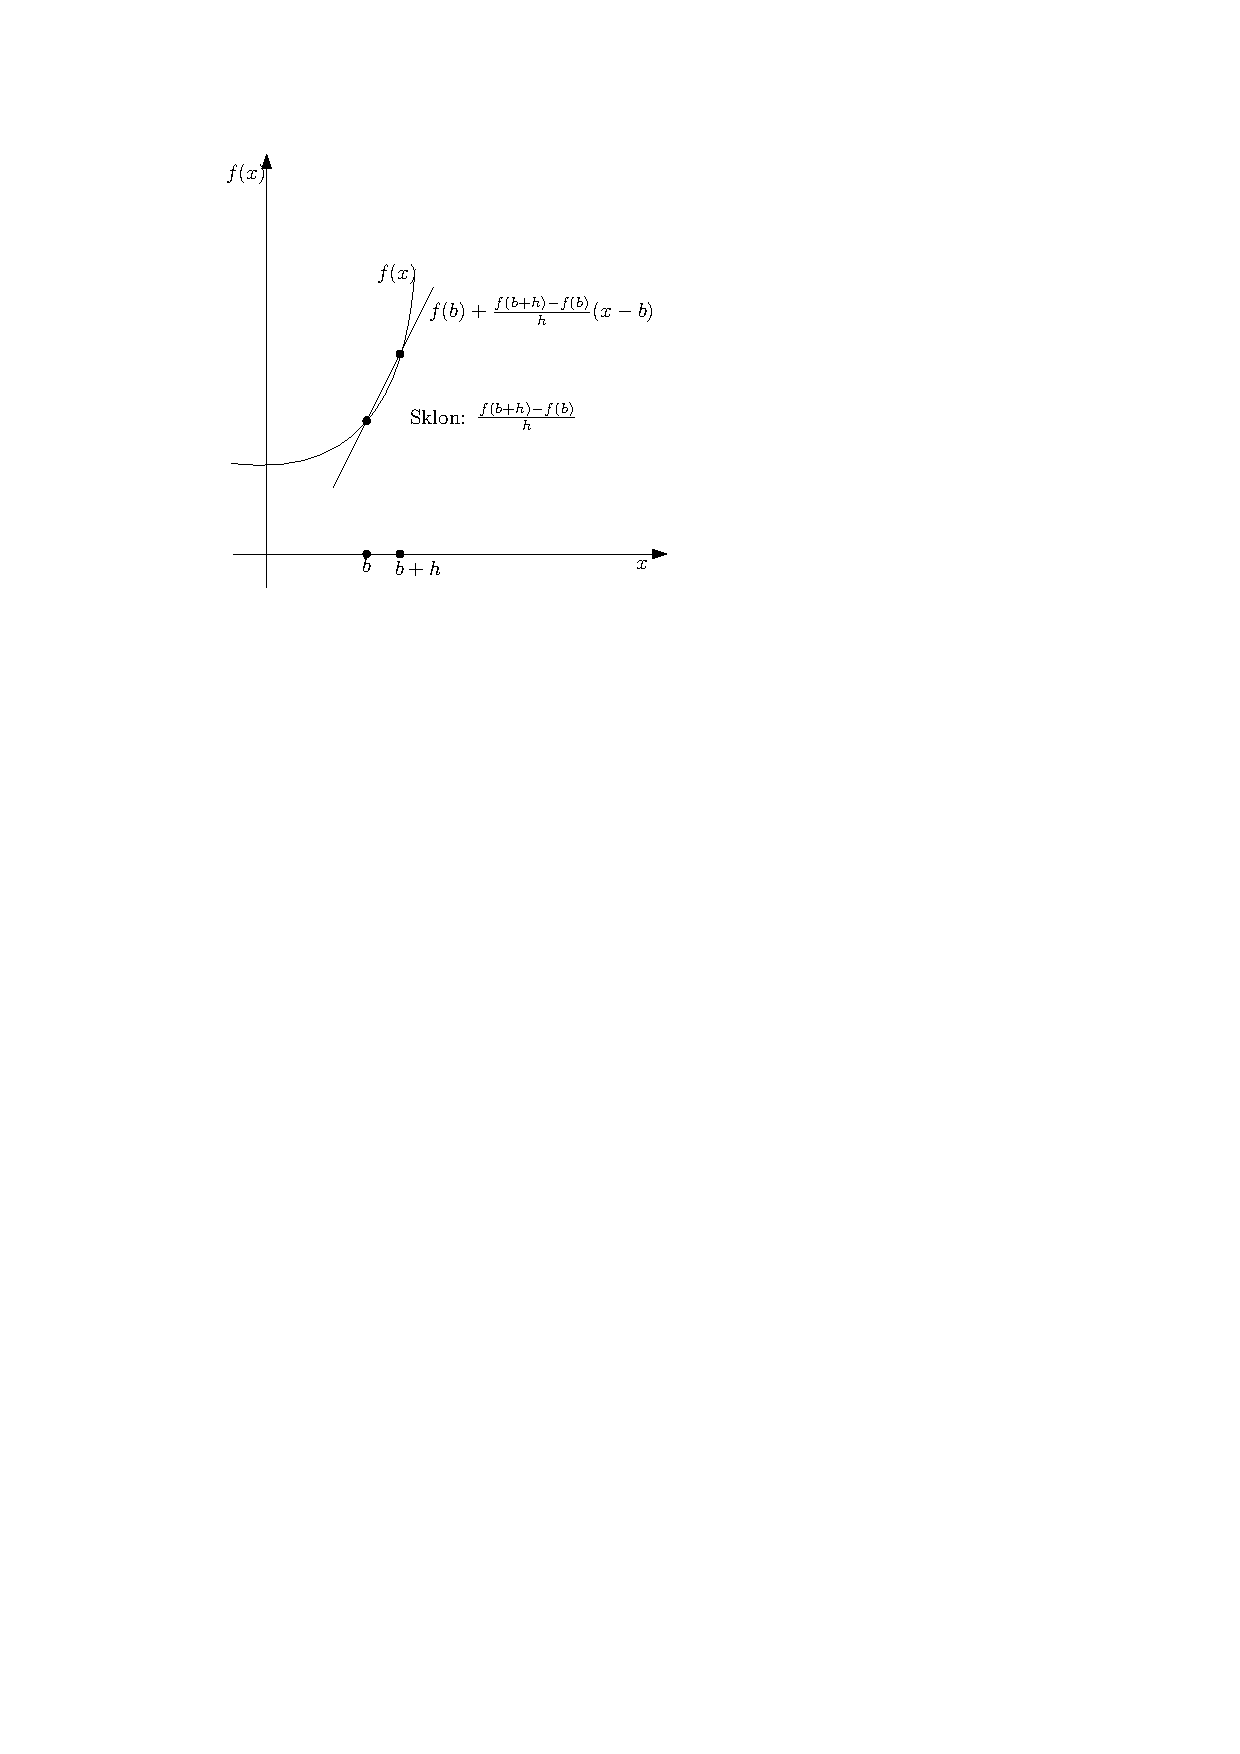
\includegraphics{tahaky/fig/derivace.pdf}
	\caption{Definice derivace v obrázku pro pevné $h$}
	\label{fig:def:derivace}
\end{figure}



	  \begin{theorem}
	O derivacích víte následující:
	\begin{enumerate}
		\item  $c' = 0$ (derivace konstanty je nula) \label{poucka:derivace_konstanty}
		\item  $(x^k)' = k x^{k-1}$ pro libovolné $k \in \mathbb{R}$ kdykoliv je toto definováno (bacha na dělení nulou při derivaci $(x^{1/2})' = \frac{1}{\sqrt{x}}$) \label{poucka:derivace_monomu}
		\item  $\sin'(x) = \cos(x)$ \label{poucka:derivace_sin}
		\item  $\cos'(x) = -\sin(x)$ \label{poucka:derivace_cos}
		\item  $\ln'(x) = 1/x$ pro $x>0$ \label{poucka:derivace_ln}
		\item  $\left( \frac{f(x)}{g(x)} \right)' = \frac{f'(x)g(x) - f(x)g'(x)}{g(x)^2}$ kdekoliv $g(x) \neq 0$
		\item  $(e^x)' = e^x$ \label{poucka:derivace_exponencialy}
		\item  Derivace je lineární operátor, tedy $(\alpha f + \beta g)'(x) = \alpha f'(x) + \beta g'(x)$ pokud je pravá strana definována \label{poucka:derivace_je_linearni_operator}
		\item  $(f\cdot g)'(x) = f'(x) g(x) + f(x) g'(x)$ pokud je pravá strana definována a $f$ nebo $g$ je spojitá \label{poucka:derivace_soucinu}
		\item  $(f\circ g)'(x) = f'(g(x)) g'(x)$ pokud je pravá strana definována, $g, f$ mají derivaci a $g$ je spojitá \label{poucka:derivace_slozene_fce}
	\end{enumerate}
	\label{thm:poucky_o_derivacich}
\end{theorem}


	\section{Taylor} \label{sec:taylor}
	  \begin{definition}[Taylorův polynom]
	Nechť $a \in \mathbb{R}$, $n \in \mathbb{N}$, $f$ je funkce definovaná na nějakém okolí $a$, která má v $a$ vlastní $n$-tou derivaci $f^{(n)}(a) \in \mathbb{R}$.
	Taylorův polynom řádu $n$ v bodě $a$ je následující polynom:
	$$T_n^{f,a}(x) = f(a) + \sum_{i = 1}^{n} \frac{f^{(i)}(a)}{i!} (x - a)^{i}$$
	\label{def:tayloruv_polynom}
\end{definition}

\begin{definition}[Taylorova řada]
	Nechť funkce $f$ definovaná na nějakém okolí $a \in \mathbb{R}$ má vlastní derivaci všech řádů v $a$.
	Pak Taylorovou řadou v $x \in \mathbb{R}$ rozumíme následující řadu:
	$$T^{f,a}(x) = f(a) + \sum_{n = 1}^{\infty} \frac{f^{(n)}(a)}{n!} (x - a)^{n}$$
	\label{def:taylorova_rada}
\end{definition}


	\section{l'Hospital}
	  \begin{theorem}[l'Hospitalovo pravidlo]
	Nechť $a \in \mathbb{R}^*$,
	nechť pro nějaké $\delta > 0$ mají dvě funkce $f, g \colon P(a, \delta) \rightarrow \mathbb{R}$ vlastní derivaci,
	nechť navíc $g'(x) \neq 0$ pro všechna $x \in P(a, \delta)$.
	\label{thm:lhospital}

	\begin{enumerate}

		\item  \emph{\uv{Případ $\frac{0}{0}$}}
			Jestliže
			$$\lim_{x \rightarrow a}f(x) = \lim_{x \rightarrow a}g(x) = 0$$
			a navíc
			$$\lim_{x \rightarrow a} \frac{f'(x)}{g'(x)} = A \in \mathbb{R}^*$$
			(limita podílu derivací existuje) pak platí:
			$$\lim_{x \rightarrow a} \frac{f(x)}{g(x)} = \lim_{x \rightarrow a} \frac{f'(x)}{g'(x)}.$$

		\item  \emph{\uv{Případ $\frac{\pm \infty}{\pm \infty}$}}
			Nebo pokud
			$$\lim_{x \rightarrow a}|g(x)| = \infty$$
			a navíc
			$$\lim_{x \rightarrow a} \frac{f'(x)}{g'(x)} = A \in \mathbb{R}^*$$
			(limita podílu derivací existuje) pak platí:
			$$\lim_{x \rightarrow a} \frac{f(x)}{g(x)} = \lim_{x \rightarrow a} \frac{f'(x)}{g'(x)}.$$

	\end{enumerate}

	Totéž platí pro jednostranné limity $x \rightarrow a^+$, $x \rightarrow a^-$.
\end{theorem}

	\section{Integrály}
	  \begin{theorem}
	Nechť $F$ je primitivní funkce k $f$
	a nechť $G$ je primitivní funkce k funkci $g$
	na nějakém intervalu $I$.
	Nechť $\alpha, \beta \in \mathbb{R}$ jsou dvě čísla.
	Pak:
	$$\int \alpha f(x) + \beta g(x) \dx = \alpha F(x) + \beta G(x)$$
	\label{thm:integral_linearni_kombinace}
\end{theorem}

\begin{theorem}[O substituci]
	Mějme funkce
	$$\varphi \colon (\alpha, \beta) \rightarrow (a, b)$$
	$$f \colon (a, b) \rightarrow \mathbb{R}$$
	přičemž $\varphi$ má na $(\alpha, \beta)$ vlastní derivaci.

	Nechť $F \colon (a, b) \rightarrow \mathbb{R}$ je primitivní funkcí k $f$ na intervalu $(a, b)$.
	Pak na intervalu $(\alpha, \beta)$ platí, že
	$$\int f(\varphi(t)) \varphi'(t) \dt = F(\varphi(t)) + c$$
	\label{thm:integral_veta_o_substituci}
\end{theorem}

\begin{theorem}[Integrace per partes]
	Nechť jsou funkce $f, g$ spojité na intervalu $(a, b)$ a funkce $F, G$ jsou k nim na $(a, b)$ primitivní.
	Potom i funkce $Fg$, $fG$ mají na intervalu $(a, b)$ primitivní funkci a tamtéž platí identita:
	$$\int f(x) G(x) \dx + \int F(x) g(x) \dx = F(x) G(x) + c$$
	\label{thm:integrace_per_partes}
\end{theorem}


	\subsection{Délka křivky, objem a povrch rotačních těles}
	  \begin{theorem}[Délka křivky]
	Nechť $f \colon [a, b] \rightarrow \mathbb{R}$ má na $[a, b]$ spojitou první derivaci.
	Pak graf funkce $f$ na intervalu $[a, b]$ má délku:
	$$\text{délka}\left( \left\{ (x, f(x)) \in \mathbb{R}^2 \mid a \leq x \leq b \right\} \right) = \int_{a}^{b} \sqrt{1 + (f'(x))^2} \dx$$
	\label{thm:delka_krivky}
\end{theorem}

\begin{theorem}[Objem rotačního tělesa]
	Nechť $f \colon [a, b] \rightarrow \mathbb{R}$ je Riemannovsky integrovatelná a nezáporná na $[a, b]$.
	Pak objem rotačního tělesa vzniklého rotací rovinného útvaru mezi $f$ a osou $x$ okolo osy~$x$
	$$V = \left\{ \left( x, y, z \right) \mid a \leq x \leq b \wedge \sqrt{y^2 + z^2} \leq f(x) \right\}$$
	je
	$$\text{objem}(V) = \pi \int_{a}^{b} f^{2}(t) \dt.$$
	\label{thm:objem_rotacniho_telesa}
\end{theorem}

\begin{theorem}[Povrch rotačního tělesa]
	Nechť $f \colon [a, b] \rightarrow \mathbb{R}$ je Riemannovsky integrovatelná a nezáporná na $[a, b]$.
	Pak povrch pláště rotačního tělesa vzniklého rotací rovinného útvaru mezi $f$ a osou $x$ okolo osy~$x$
	$$V = \left\{ \left( x, y, z \right) \mid a \leq x \leq b \wedge \sqrt{y^2 + z^2} \leq f(x) \right\}$$
	je
	$$\text{povrch pláště}(V) = 2 \pi \int_{a}^{b} f(t) \sqrt{1 + (f'(t))^2} \dt$$
	\label{thm:povrch_rotacniho_telesa}
\end{theorem}


	\subsection{Odhady a řady}
	  \begin{theorem}[Odhad součtu pomocí integrálu]
	Nechť $n \in \mathbb{N}$, nechť funkce $f$ je neklesající na intervalu $[1, n]$.
	Pak platí:
	$$\sum_{k = 1}^{n-1} f(k) \leq \int_{1}^{n} f(x) \dx \leq \sum_{k = 2}^{n} f(k)$$
	\label{thm:odhad_souctu_integralem}
\end{theorem}

\begin{theorem}[Integrální kritérium konvergence]
	Nechť $f \colon [1, \infty) \rightarrow [0, +\infty)$ je nerostoučí nezáporná funkce.
	Potom řada $\sum_{k = 1}^{\infty} f(k)$ konverguje právě tehdy když
	$$\lim_{b \rightarrow \infty} \int_{1}^{b} f(x) \dx < +\infty$$
	\label{thm:integralni_kriterium_konvergence}
\end{theorem}



\chapter{Řešení}
	% solution macro, this prints the solution
	\renewcommand{\solution}[1]{
		{\normalfont
			\textbf{\emph{Řešení:}}
			#1
		}
	}
	\renewcommand{\exercise}[2]{ % file, label
		\textbf{
			\label{sol:#2}
			\input{#1}
			\newpage
		}
	}
	\section[1. Cvičení]{Cvičení}
 \include*{s1}
	\section[2. Cvičení]{Cvičení}
 \include*{s2}
	\section[3. Cvičení]{Cvičení}
 \include*{s3}
	\section[4. Cvičení]{Cvičení}
 \include*{s4}
	\section[5. Cvičení]{Cvičení}
 \include*{s5}
	\section[6. Cvičení]{Cvičení}
 \include*{s6}
	\section[7. Cvičení]{Cvičení}
 \include*{s7}
	\section[8. Cvičení]{Cvičení}
 \include*{s8}
	\section[9. Cvičení]{Cvičení}
 \include*{s9}
	\section[10. Cvičení]{Cvičení}
 \include*{s10}
	\section[11. cvičení]{cvičení}
 \include*{s11}
	\section[12. cvičení]{cvičení}
 \include*{s12}
	\section[13. cvičení]{cvičení}
 \include*{s13}
	\section[14. cvičení]{cvičení}
 \include*{s14}

\chapter{Řešení vybraných domácích úkolů}

\begin{enumerate}
	\item  \exercise{homework/charakterizace_kdy_omezena_nema_limitu.tex}{hw_charakterizace_nema_limitu}
	\item  \exercise{homework/rekurentni.tex}{hw_rekurentni}
	\item  \exercise{homework/spojitost_odmocniny.tex}{hw_spojitost_odmocniny}
	\item  \exercise{homework/limity.tex}{hw_limity}
	\item  \exercise{homework/darboux.tex}{hw_darboux}
	\item  \exercise{homework/podilove_kriterium.tex}{hw_podilove_kriterium}
	\item  \exercise{homework/kvizy_4_az_9.tex}{hw_kvizy}
\end{enumerate}

\chapter{Bonus}

\section{Optimalizace -- gradient descend}
Už jsme viděli, jak použít Darbouxovu vlastnost a \uv{půlení intervalů} na optimalizaci.
Ale to nemusí být vždy praktické:
\begin{itemize}

	\item  Rychlost konvergence\ldots

	\item  Jak ten postup zobecníte na funkce více proměnných?

\end{itemize}

Zkusme se podívat na následující funkci a najít její minimum fyzikální úvahou:
$$f(x) = x^4 - 3x^3 + 2$$

Analytickými metodami umíme snadno najít minimum (vyšetříme první a druhé derivace, vzpomeneme si na věty z přednášky a jsme hotovi).
(Obrázek~\ref{fig:gradient_descend}).
\begin{figure}[H]
	\centering
	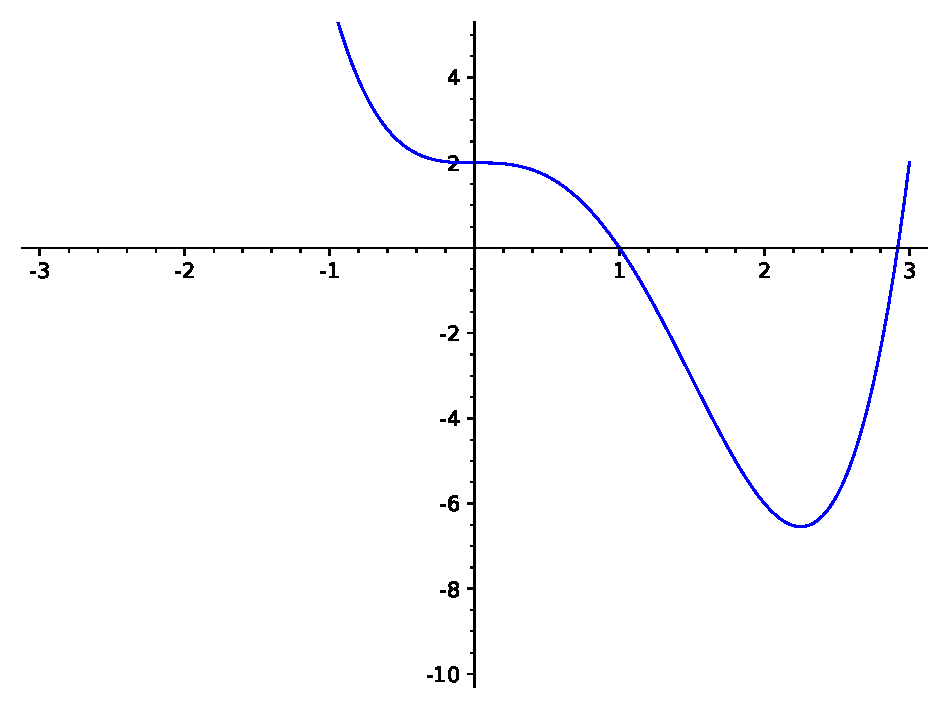
\includegraphics{bonus/fig/gd.pdf}
	\caption{$f(x) = x^4 - 3x^3 + 2$}
	\label{fig:gradient_descend}
\end{figure}

\textbf{Myšlenka:} co by se stalo, kdybychom po grafu pustili kuličku?

\textbf{Pozorování:} skutálí se dolů do minima!

\textbf{Otázka:} ale kudy je dolů?

Derivaci téhle funkce umíme vyhodnotit snadno: $f'(x) = 4x^3 - 9x^2$.
\begin{itemize}
	\item  Pokud je derivace záporná, funkce klesá.
	\item  Pokud je derivace kladná, funkce roste.
\end{itemize}

Dokonce platí něco lepšího:
\begin{itemize}
	\item  Pokud je derivace \emph{hodně} záporná, funkce \emph{hodně} klesá.
	\item  Pokud je derivace \emph{hodně} kladná, funkce \emph{hodně} roste.
\end{itemize}

Takže když chceme minimalizovat, děláme tohle:
\begin{itemize}
	\item  Pokud je derivace (hodně) kladná, jdeme (hodně) vlevo.
	\item  Pokud je derivace (hodně) záporná, jdeme (hodně) vpravo.
\end{itemize}

To zní dobře, protože v extrému je derivace nulová (nebo neexistuje, ale to teď zanedbáme), takže se nepohneme nikam.

Jednodušeji řečeno: odečteme derivaci.

Jednoduchý Python kód:
\inputminted{python}{bonus/gd.py}
Výstup:
\texttt{\\
current = 4.0\\
current = 2.88\\
current = 2.67098112\\
current = 2.55084758768784\\
current = 2.4725451025639247\\
current = 2.4181241075908217\\
current = 2.3788010610759907\\
current = 2.349647226900712\\
current = 2.3276417627201864\\
current = 2.3108155002345616\\
current = 2.297825629818595\\
current = 2.2877248517791187\\
current = 2.279827252147626\\
current = 2.2736260324425532\\
current = 2.2687407592672773\\
current = 2.2648822733430056\\
current = 2.2618286143740107\\
current = 2.2594080688614797\\
current = 2.2574869694912945\\
current = 2.2559607515339213\\
Minimum at: 2.254747295376156
}

Připomeňme, že skutečné minimum je 2.25.

\emph{
	Zkuste si pohrát s tím kódem.
}
Problémy, které mohou nastat:
\begin{itemize}

	\item  Zasekneme se v inflexním bodě. Tohle se snad nestane (\uv{vratká pozice}).

	\item  Příliš velké alpha můžeme ulítnout (poskakujeme zleva doprava čím dál tím větší skoky).
		Tohle bývá problém, proto se občas postupně snižuje alpha, ke kroku se přičte i nějaký malý násobek předchozího kroku\ldots
		Spousta heuristik, které běží lépe.
		Nad rámec tohoto povídání.

	\item  Málo iterací -- no tak poběžíme více iterací (tzn. déle).

\end{itemize}


\section{Nikdo neočekává, že tohle budete číst (a na cvičení se tomu taky nebudeme věnovat): Jednoduchá neuronka}
\subsection{Problém, který budeme řešit}

Naše neuronka bude řešit klasický problém, z daného obrázku (28 krát 28 pixelů, 256 odstínů šedé) budeme chtít určit, která ručně psaná číslice je na něm napsaná.

Data si můžeme stáhnout z \url{http://yann.lecun.com/exdb/mnist/} kde máme popis formátu dat a některé známé metody strojového učení a jejich výsledky.
My se nebudeme snažit dosáhnout co nejlepšího výsledku (ale dostaneme celkem dobrý výsledek).

Data jsou rozdělena do 60000 obrázků a příslušných 60000 labelů (správných číslic) na trénování a 10000 obrázků a labelů na testování.
To je důležité, nakonec chceme zjistit, jak dobře naše neuronka odpovídá na datech, která ještě před tím nikdy neviděla (nechceme memorizovat, ale generalizovat naučené).

\subsection{Struktura neuronové sítě}

\paragraph{Vstup}
Vstupem bude obrázek $28 \times 28$ pixelů.
Pro lepší manipulaci si ho přeuspořádáme do vektoru $x \in \mathbb{R}^{784}$ (například po jednotlivých řádcích).

\paragraph{Výstup}
Výstupem by intuitivně měla být ta číslice, která je na obrázku na vstupu.
Ale co když nebude jasné, jestli na vstupu je jednička nebo sedmička (ručně psané se mohou plést).
Asi bychom nechtěli, aby síť vystoupila \uv{něco mezi}, tedy třeba čtyřku.
Proto bude síť vystupovat pravděpodobnostní distribuci $y \in \mathbb{R}^{10}$ (kde $0 \leq y_i \leq 1$ a navíc $\sum_{i = 0}^{9} y_i = 1$).
Interpretujeme to tak, že na obrázku je nula s pravděpodobností $y_0$, na obrázku je jednička s pravděpodobností $y_1$, \ldots, devítka s pravděpodobností $y_9$.
Pokud chceme výsledek jedno číslo, tak zvolíme ten index, který má největší pravděpodobnost (argmax).

Často se nám hodí \uv{zmenšit} velká čísla na malá (nebudeme mít chyby způsobené tím, že některé číslo bude příliš velké).
Dále pak potřebujeme nějakou nelinearitu (afinní zobrazení nejsou dostatečně obecná).
Na to se hodí následující funkce, které se říká sigmoid:
$$\sigma(x) = \frac{1}{1 + e^{-x}}$$
\todo{obrázek sigmoid}

Vstup ještě můžeme \uv{zmáčknout} jednoduše tím, že vydělíme 255.

Jak tedy vypadá naše síť?

\begin{itemize}

  \item  Reprezentace vstupního obrázku:
    $$x \in \mathbb{R}^{784}$$

  \item  První afinní funkce:
    $$z^{(1)} = W^{(1)} x + b^{(1)} \in \mathbb{R}^{100}$$
    kde indexujeme nahoře, protože dolní indexy se nám budou hodit, tedy $W^{(1)} \in \mathbb{R}^{100 \times 784}$ je jen obyčejná matice a $b^{(1)} \in \mathbb{R}^{100}$ je vektor.

  \item  Jedna skrytá vrstva neuronů:
    $$a^{(1)} = \sigma(z^{(1)}) \in \mathbb{R}^{100}$$
    kde jen aplikujeme sigmoid na každé číslo vektoru $z^{(1)}$.

  \item  Druhá afinní funkce:
    $$z^{(2)} = W^{(2)} x + b^{(2)} \in \mathbb{R}^{10}$$
    kde $W^{(2)} \in \mathbb{R}^{10 \times 100}$ a $b^{(2)} \in \mathbb{R}^{10}$.

  \item  Z výsledku druhé afinní funkce uděláme pravděpodobnostní distribuci pomocí softmax:
    $$(\hat{y})_i = \frac{e^{z^{(2)}_i}}{ \sum_{i=1}^{10} e^{z^{(2)}_i} }$$
    Tedy $\hat{y} \in \mathbb{R}^{10}$ je pravděpodobnostní distribuce ($e^x$ je nezáporná, podělíme to součtem).

\end{itemize}

Známe obrázek $x$, známe příslušný 1-hot vektor, který měl vyjít jako $\hat{y}$ (pokud číslice byla tři, mělo vyjít $\hat{y} = (0, 0, 0, 1, 0, 0, 0, 0, 0, 0)^T$).
Jak ale určíme parametry $W^{(1)}, b^{(1)}, W^{(2)}, b^{(2)}$?
Můžeme je zvolit náhodně a pak zkusit minimalizovat vzdálenost $\hat{y}$ od skutečného $y$.

Budeme minimalizovat něco, čemu se říká cross-entropy (protože to je zajímavá vzdálenost dvou pravděpodobnostních distribucí a máme rádi teorii informace a Claude Shannon to nevymyslel zbytečně).
$$L(y, \hat{y}) = -\sum_{i = 1}^{10} y_i \log(\hat{y_i})$$

Výhodou je, že $L(y, \hat{y})$ je jedno reálné číslo, které můžeme minimalizovat.

\subsection{Učení}

Pokud číslo $L(y, \hat{y})$ bereme jako funkci například $W^{(1)}_{1, 1}$ (tj. číslo $W^{(1)}_{1, 1}$ je proměnná, zbytek parametrů jsou konstanty).
Teď se můžeme ptát, jak moc se změní $L$, když o trošku změníme $W^{(1)}_{1, 1}$.
Tedy nás zajímá derivace $L$ podle $W^{(1)}_{1, 1}$ tu budeme zapisovat Leibnitzovou notací jako $\frac{dL}{dW^{(1)}_{1, 1}}$.

Protože máme spoustu složených funkcí, budeme využívat poučku o derivaci složené funkce.
Tvar, na který jsme zvyklí je:
$$(f(g(x)))' = f'(g(x))g'(x)$$
v Leibnitzově notaci to bude pak:
$$\frac{dz}{dx} = \frac{dz}{dy}\frac{dy}{dx}$$
kde $x$ je proměnná, podle které derivujeme, $y = g(x)$, $z = f(y)$.

No a tohle chceme spočítat pro každý parametr a pak udělat gradient descend.

\subsection{Učení, když bychom měli jen pár parametrů}

Mohli bychom rovnou zkusit odvodit pro každý parametr zvlášť jak ho změnit, ale jednodušší to bude, když budeme vše držet ve vektorech a maticích.

Představme si, že vstupní obrázek má jen dva pixely, výstup jsou jen dvě třídy (tedy pravděpodobnost $p, 1-p$) a vnitřní vrstva je taky dva neurony.
Postupně odvodíme derivace.

\begin{itemize}

  \item  Reprezentace vstupního obrázku:
    $$x =
    \begin{pmatrix}
      x_1 \\
      x_2
    \end{pmatrix}
    \in \mathbb{R}^{2}$$

  \item  První afinní funkce:
    $$z^{(1)} =
    \begin{pmatrix}
      z^{(1)}_1 \\
      z^{(1)}_2
    \end{pmatrix}
    = W^{(1)} x + b^{(1)} =
    \begin{pmatrix}
      W^{(1)}_{1, 1} & W^{(1)}_{1, 2} \\
      W^{(1)}_{2, 1} & W^{(1)}_{2, 2} 
    \end{pmatrix}
    \begin{pmatrix}
      x_1 \\
      x_2
    \end{pmatrix}
    +
    \begin{pmatrix}
      b^{(1)}_1 \\
      b^{(1)}_2
    \end{pmatrix}
    $$

  \item  Jedna skrytá vrstva neuronů:
    $$a^{(1)} = \sigma(z^{(1)}) =
    \begin{pmatrix}
      \sigma(z^{(1)}_1) \\
      \sigma(z^{(1)}_2)
    \end{pmatrix}
    \in \mathbb{R}^{2}$$

  \item  Druhá afinní funkce:
    $$z^{(2)} = W^{(2)} x + b^{(2)} = 
    \begin{pmatrix}
      W^{(2)}_{1, 1} & W^{(2)}_{1, 2} \\
      W^{(2)}_{2, 1} & W^{(2)}_{2, 2} 
    \end{pmatrix}
    \begin{pmatrix}
      a^{(1)}_1 \\
      a^{(1)}_2
    \end{pmatrix}
    +
    \begin{pmatrix}
      b^{(2)}_1 \\
      b^{(2)}_2
    \end{pmatrix}
    \in \mathbb{R}^{2}$$

  \item  Z výsledku druhé afinní funkce uděláme pravděpodobnostní distribuci pomocí softmax:
    $$(\hat{y})_i = 
    \begin{pmatrix}
     \frac{e^{z^{(2)}_1}}{ \sum_{i=1}^{2} e^{z^{(2)}_i} } \\
     \frac{e^{z^{(2)}_2}}{ \sum_{i=1}^{2} e^{z^{(2)}_i} }
    \end{pmatrix}
    \in \mathbb{R}^2
    $$

  \item  Chceme minimalizovat ztrátu:
    $$L(\hat{y}, y) =
    -y_1 \log(\hat{y_1}) - y_2 \log(\hat{y_2})
    \in \mathbb{R}
    $$

\end{itemize}

Připomeňme, že $x, y$ je obrázek a daný label, tedy čísla, která známe.

\subsubsection{Derivování a skládání do matic a vektorů}

Vektorový kalkulus sice ještě neznáme, ale nebude tak těžké ho odvodit.
Pro řetízkové pravidlo bychom chtěli vědět, jak moc máme pohnout vektor
$
\begin{pmatrix}
  z^{(2)}_1 \\
  z^{(2)}_2
\end{pmatrix}
$
abychom zmenšili ztrátu $L$.

\begin{itemize}

  \item  Pro řetízkové pravidlo chceme \uv{derivaci $L$ podle $z^{(2)}$}.
    Tedy chceme spočítat
    $
    \begin{pmatrix}
      \frac{dL}{d z^{(2)}_1} \\
      \frac{dL}{z^{(2)}_2}
    \end{pmatrix}
    $
    \begin{align*}
    \begin{pmatrix}
      \frac{dL}{d z^{(2)}_1} \\
      \frac{dL}{z^{(2)}_2}
    \end{pmatrix}
    &=
    \begin{pmatrix}
      \frac{dL}{d\hat{y_1}}\frac{d\hat{y_1}}{d z^{(2)}_1} + \frac{dL}{d\hat{y_2}}\frac{d\hat{y_2}}{d z^{(2)}_1} \\
      \frac{dL}{d\hat{y_1}}\frac{d\hat{y_1}}{z^{(2)}_2} + \frac{dL}{d\hat{y_2}}\frac{d\hat{y_2}}{z^{(2)}_2}
    \end{pmatrix} \\
    &=
    \begin{pmatrix}
      -\frac{y_1}{\hat{y_1}} \left( \hat{y_1}(1 - \hat{y_1}) \right) + \frac{y_2}{\hat{y_2}} \left( - \hat{y_1}\hat{y_2} \right) \\
      -\frac{y_1}{\hat{y_1}} \left( - \hat{y_1}\hat{y_2} \right) + \frac{y_2}{\hat{y_2}} \left( \hat{y_2}(1 - \hat{y_2}) \right)
    \end{pmatrix} \\
    &=
    \begin{pmatrix}
      \hat{y_1}(y_1 + y_2) - y_1 \\
      \hat{y_2}(y_1 + y_2) - y_2 
    \end{pmatrix} \tag{$y_1 + y_2 = 1$ prst. distrib.} \\
    &=
    \begin{pmatrix}
      \hat{y_1} - y_1 \\
      \hat{y_2} - y_2 
    \end{pmatrix}
    \end{align*}

  \item  Ale $z^{(2)}$ není parametr, ten nemůžu změnit, ale $W^{(2)}$ můžu změnit pomocí gradient descend, tedy chci \uv{derivaci $L$ podle $W^{(2)}$}.
    Pomocí řetízkového pravidla tedy spočítám gradient.
    V následujícím píšu $w_{i,j}$ místo $w^{(2)}_{i,j}$ a $z_i$ místo $z^{(2)}_i$ a $a_i$ místo $a^{(1)}_i$, abych tam neměl tolik indexů.
    \begin{align*}
      \begin{pmatrix}
        \frac{dL}{dw_{1,1}}  & \frac{dL}{dw_{1,2}} \\
        \frac{dL}{dw_{2,1}}  & \frac{dL}{dw_{2,2}}
      \end{pmatrix}
      &=
      \begin{pmatrix}
        \frac{dL}{dz_1}\frac{dz_1}{dw_{1,1}}  & \frac{dL}{dz_1}\frac{dz_1}{dw_{1,2}} \\
        \frac{dL}{dz_2}\frac{dz_2}{dw_{2,1}}  & \frac{dL}{dz_2}\frac{dz_2}{dw_{2,2}}
      \end{pmatrix} \tag{$z_2$ není funkcí $w_{1,2}$} \\
      &=
      \begin{pmatrix}
        (\hat{y_1} - y_1)a_1 & (\hat{y_1} - y_1) a_2 \\
        (\hat{y_2} - y_2)a_1 & (\hat{y_2} - y_2) a_2
      \end{pmatrix} \\
      &=
      \begin{pmatrix}
        \hat{y_1} - y_1 \\
        \hat{y_2} - y_2 
      \end{pmatrix}
      \begin{pmatrix}
        a_1 & a_2
      \end{pmatrix}
    \end{align*}

  \item  Další parametr, který můžeme měnit dle gradient descend je $b^{(2)}$ opět vynechávám horní indexy.
    \begin{align*}
      \begin{pmatrix}
        \frac{dL}{db_1} \\
        \frac{dL}{db_2} 
      \end{pmatrix}
      &=
      \begin{pmatrix}
        \frac{dL}{dz_1}\frac{dz_1}{db_1} \\
        \frac{dL}{dz_2}\frac{dz_2}{db_2} 
      \end{pmatrix} \\
      &=
      \begin{pmatrix}
        \hat{y_1} - y_1 \\
        \hat{y_2} - y_2 
      \end{pmatrix} 
    \end{align*}

  \item  Opět výpočet čistě pro řetízkové pravidlo \uv{derivace $L$ podle $a^{(1)}$}.
    Pozor na to, že $L$ závisí na $z^{(2)}_1$ i $z^{(2)}_2$ a oboje závisí na $a^{(1)}_1$, tedy použijeme linearitu
    \begin{align*}
      \begin{pmatrix}
        \frac{dL}{da_1} \\
        \frac{dL}{da_2}
      \end{pmatrix}
      &=
      \begin{pmatrix}
        \frac{dL}{dz1}\frac{dz_1}{da_1} + \frac{dL}{dz_2}\frac{dz_2}{da_1} \\
        \frac{dL}{dz1}\frac{dz_1}{da_2} + \frac{dL}{dz_2}\frac{dz_2}{da_2}
      \end{pmatrix} \\
      &=
      \begin{pmatrix}
        (\hat{y_1} - y_1)w_{1,1} + (\hat{y_2} - y_2)w_{2,1} \\
        (\hat{y_1} - y_1)w_{1,2} + (\hat{y_2} - y_2)w_{2,2}
      \end{pmatrix} \\
      &=
      \begin{pmatrix}
        w_{1,1} & w_{2,1} \\
        w_{1,2} & w_{2,2}
      \end{pmatrix}
      \begin{pmatrix}
        \hat{y_1} - y_1 \\
        \hat{y_2} - y_2 
      \end{pmatrix} \\
      &=
      (W^{(1)})^T
      \begin{pmatrix}
        \hat{y_1} - y_1 \\
        \hat{y_2} - y_2 
      \end{pmatrix}
    \end{align*}

  \item  Teď spočítáme podle $z^{(1)}$, na to napřed potřebujeme zderivovat sigmoid:
    $$\left( \frac{1}{1+e^{-x}} \right)' = \frac{e^{-x}}{1 + e^{-x}} = \sigma(x)(1-\sigma(x))$$
    \begin{align*}
      \begin{pmatrix}
        \frac{dL}{dz_1} \\
        \frac{dL}{dz_2}
      \end{pmatrix}
      &=
      \begin{pmatrix}
        \frac{dL}{da_1}\frac{da_1}{dz_1} \\
        \frac{dL}{da_2}\frac{da_2}{dz_2}
      \end{pmatrix} \\
      &=
      \begin{pmatrix}
        \frac{dL}{da_1} \sigma(z_1)(1-\sigma(z_1)) \\
        \frac{dL}{da_2} \sigma(z_2)(1-\sigma(z_2))
      \end{pmatrix}
    \end{align*}
    Ten poslední výraz by se dal zapsat pomocí Hadamardova násobení matic (tam násobíme jen příslušné prvky).

  \item  Analogicky spočítáme gradient pro $W^{(1)}$:
    \begin{align*}
      \begin{pmatrix}
        \frac{dL}{dw_{1,1}} & \frac{dL}{dw_{1,2}} \\
        \frac{dL}{dw_{2,1}} & \frac{dL}{dw_{2,2}} \\
      \end{pmatrix}
      &=
      \begin{pmatrix}
        \frac{dL}{dz_1} \\
        \frac{dL}{dz_2}
      \end{pmatrix}
      \begin{pmatrix}
        x_1 & x_2
      \end{pmatrix}
    \end{align*}

  \item  Analogicky spočítáme gradient pro $b^{(1)}$:
    \begin{align*}
      \begin{pmatrix}
        \frac{dL}{db_1} \\
        \frac{dL}{db_2}
      \end{pmatrix}
      &=
      \begin{pmatrix}
        \frac{dL}{dz_1} \\
        \frac{dL}{dz_2}
      \end{pmatrix}
    \end{align*}

\end{itemize}

Příslušné gradienty můžeme odčítat v gradient descend.

\subsection{Kód}

Jednoduchý python kód.
Používáme jen numpy, vynechali jsme čtení vstupu a vyhodnocování přesnosti.

\inputminted{python}{bonus/nn_jen_uceni.py}



\end{document}
